% Basic stuff
\documentclass{article}
\usepackage[utf8]{inputenc}
\usepackage[a4paper, total={6.5in, 9.5in}]{geometry}
\usepackage[bookmarks, hidelinks, unicode]{hyperref}
\usepackage[]{amsmath,amssymb}
\usepackage{stmaryrd}
\usepackage{tikz}
\usepackage{lmodern}
\usepackage{soul}
\usepackage{float}

% Packages configuration
\usetikzlibrary{shapes.arrows, angles, quotes}
\renewcommand{\arraystretch}{1.4}
\restylefloat{table}

% Shortcut commands
\newcommand{\im}{\text{Im}\,}
\newcommand{\re}{\text{Re}\,}
\newcommand{\img}{\text{Img}\,}
\newcommand{\R}{{\mathbb R}}
\newcommand{\Y}{{\mathbb Y}}
\newcommand{\FEF}[1]{\underset{f:A\to B}{\text{FEF}}#1}
\renewcommand{\C}{{\mathbb C}}
\newcommand{\N}{{\mathbb N}}
\newcommand{\Z}{{\mathbb Z}}
\newcommand{\Q}{{\mathbb Q}}
\renewcommand{\U}{{\mathbb U}}
\newcommand{\cC}{{\mathcal C}}
\newcommand{\cD}{{\mathcal D}}
\newcommand{\cF}{{\mathcal F}}
\newcommand{\cP}{{\mathcal P}}
\newcommand{\cL}{{\mathcal L}}
\newcommand{\cotan}{\operatorname{cotan}}
\newcommand{\conj}[1]{\overline{#1}}
\newcommand{\Aff}{\text{Aff}}
\newcommand{\twoRows}[1]{\multirow{2}{*}{#1}}
\newcommand{\threeRows}[1]{\multirow{3}{*}{#1}}
\newcommand{\twoCols}[1]{\multicolumn{2}{c|}{#1}}
\newcommand{\threeCols}[1]{\multicolumn{3}{|c|}{#1}}
\newcommand{\twoColsNB}[1]{\multicolumn{2}{c}{#1}}
\newcommand{\goesto}[2]{\xrightarrow[#1\:\to\:#2]{}}
\newcommand{\liminfty}{\lim_{x\to+\infty}}
\newcommand{\limminfty}{\lim_{x\to-\infty}}
\newcommand{\limzero}{\lim_{x\to0}}
\newcommand{\const}{\text{cste}}
\newcommand{\et}{\:\text{et}\:}
\newcommand{\ou}{\:\text{ou}\:}
\newcommand{\placeholder}{\diamond}
\newcommand{\mediateur}{\:\text{med}\:}
\newcommand{\milieu}{\:\text{mil}\:}
\newcommand{\vect}[1]{\overrightarrow{#1}}
\newcommand{\point}[2]{(#1;\;#2)}
\newcommand{\spacepoint}[3]{\begin{pmatrix}#1\\#2\\#3\end{pmatrix}}
\newcommand{\sh}{\operatorname{sh}}
\newcommand{\ch}{\operatorname{ch}}
\renewcommand{\th}{\operatorname{th}}
\newcommand{\id}{\operatorname{id}}
\renewcommand{\cong}{\equiv}
\newcommand{\converges}[2]{\xrightarrow[{#1\to #2}]{}}
\newcommand{\convergedby}[2]{\xleftarrow[{#1\to #2}]{}}

\newcommand{\decreasingfunctions}{%
	\begin{tikzpicture}[scale=1.75, baseline=0]%
		\draw (0,-0.25ex) -- (1ex,-0.25ex);%
		\draw (1ex,0) arc (0:90:1ex);%
	\end{tikzpicture}\,%
}

\newcommand{\strictlydecreasingfunctions}{%
	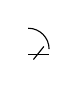
\begin{tikzpicture}[scale=1.75, baseline=0]%
		\draw (0,-0.25ex) -- (1ex,-0.25ex);%
		\draw (1ex,0) arc (0:90:1ex);%
		\draw (0.75ex,0.125ex) -- (0.25ex,-0.5ex);%
	\end{tikzpicture}\,%
}

\newcommand{\increasingfunctions}{%
	\begin{tikzpicture}[scale=1.75, baseline=0]%
		\draw (0,-0.25ex) -- (1ex,-0.25ex);%
		\draw (0,0) arc (-90:0:1ex);%
	\end{tikzpicture}\,%
}

\newcommand{\strictlyincreasingfunctions}{%
	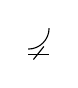
\begin{tikzpicture}[scale=1.75, baseline=0]%
		\draw (0,-0.25ex) -- (1ex,-0.25ex);%
		\draw (0,0) arc (-90:0:1ex);%
		\draw (0.75ex,0.125ex) -- (0.25ex,-0.5ex);%
	\end{tikzpicture}\,%
}
\newcommand{\strictlymonotonics}{%
	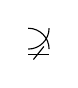
\begin{tikzpicture}[scale=1.75, baseline=0]%
		\draw (0,-0.25ex) -- (1ex,-0.25ex);%
		\draw (0,0) arc (-90:0:1ex);%
		\draw (1ex,0) arc (0:90:1ex);%
		\draw (0.75ex,0.125ex) -- (0.25ex,-0.5ex);%
	\end{tikzpicture}\,%
}
\newcommand{\periodicfunctions}{\circlearrowleft}
\newcommand{\concave}{}
\newcommand{\convexes}{}
\newcommand{\intensives}{}
\newcommand{\extensives}{}

\newcommand{\evenfunctions}{%
	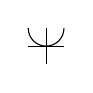
\begin{tikzpicture}[scale=1.5, baseline=-0.5ex]%
		\draw (-1ex,0) -- (1ex,0);%
		\draw (0,-1ex) -- (0, 1ex);%
		\draw (0ex, 0ex) arc (-90:0:1ex);%
		\draw (0ex, 0ex) arc (90:0:-1ex);%
	\end{tikzpicture}\,%
}

\newcommand{\oddfunctions}{%
	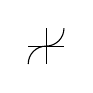
\begin{tikzpicture}[scale=1.5, baseline=-0.5ex]%
		\draw (-1ex,0) -- (1ex,0);%
		\draw (0,-1ex) -- (0, 1ex);%
		\draw (0ex, 0ex) arc (-90:0:1ex);%
		\draw (0ex, 0ex) arc (-90:0:-1ex);%
	\end{tikzpicture}\,%
}

\newcommand{\bijections}{%
	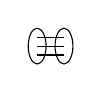
\begin{tikzpicture}[scale=1.5, baseline=-0.5ex]%
		\draw (-0.75ex,0) ellipse (0.5ex and 1ex);
		\draw (0.75ex,0) ellipse (0.5ex and 1ex);
		\draw (-0.75ex,0.5ex) -- (0.75ex,0.5ex);
		\draw (-0.75ex,0) -- (0.75ex,0);
		\draw (-0.75ex,-0.5ex) -- (0.75ex,-0.5ex);
	\end{tikzpicture}\,%
}

\newcommand{\injections}{%
	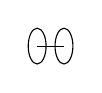
\begin{tikzpicture}[scale=1.5, baseline=-0.5ex]%
		\draw (-0.75ex,0) ellipse (0.5ex and 1ex);
		\draw (0.75ex,0) ellipse (0.5ex and 1ex);
		\draw (-0.75ex,0) -- (0.75ex,0);
	\end{tikzpicture}\,%
}

\newcommand{\surjections}{%
	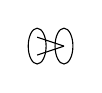
\begin{tikzpicture}[scale=1.5, baseline=-0.5ex]%
		\draw (-0.75ex,0) ellipse (0.5ex and 1ex);
		\draw (0.75ex,0) ellipse (0.5ex and 1ex);
		\draw (-0.75ex,0.5ex) -- (0.75ex,0);
		\draw (-0.75ex,-0.5ex) -- (0.75ex,0);
	\end{tikzpicture}\,%
}
% Document

\author{Ewen Le Bihan}
\date{2020-12-29}
\title{Fonctions à ensembles fonctionnels}
\begin{document}
\maketitle
\begin{abstract}
	La notation $\cD(A, B)$ désignant l'ensemble des fonctions dérivables sur $A$ de type $A\to B$ est assez commune, et facilement définissable de manière formelle, ainsi que sa généralisation, $\cD^n$, ou son homologue pour les fonctions continues, $\cC$. Mais il y a bien un lien entre ces trois notations: ce sont des \emph{fonctions à valeurs d'ensembles ne contenant que des fonctions du type correspondants aux deux arguments passés à la fonction}, ou, plus succintement, pour tous ensembles $A$ et $B$, $\cD(A, B) \in \mathcal P(\cF(A, B))$.
	
%\footnote{On remarque aussi que la notation $\cF$ est elle-même une fonction à ensembles fonctionnels}

	Dans cet article est exploré cette “classe” d'objets particuliers. On défini pour tout le reste de l'article l'abbréviation {\bf FEF}, signifiant “Fonctions à valeurs d'ensembles fonctionnels”. On note dans la suite de tout l'article $A$ et $B$ deux ensembles quelconques, $:=$ l'égalité par définition et $\text{univers}$ l'unique ensemble tel que pour tout ensemble $A$, $A \neq \text{univers} \implies A \subset \text{univers}$.
\end{abstract}

\section{Définitions}

\subsection{Définition de l'ensemble des FEF}
\paragraph{}

On définit dès lors un nouvel ensemble $\Y$%\footnote{$\Y$ est préféré à $\mathbb F$ car $\mathbb F$ désigne déjà l'ensemble des champs, et $\Y$ n'a aucun usage répertorité sur Wikipédia.

\[
	\Y := \cF(A \times B,\ \mathcal P(\cF(A, B))
\] 
Où:

\begin{itemize}
	\item $\cF$ désigne l'ensemble des fonctions de type $A\to B$. Pour la définition formelle de $\cF$, cf. \ref{formal_def_F}.
	\item $\mathcal P(A)$ désigne l'ensemble des parties de $A$
\end{itemize}

\paragraph{}
On a bien:

\begin{itemize}
	\item $\cF \in \Y$
	\item $\cC \in \Y$
	\item $\cD \in \Y$
\end{itemize}



\subsection{Un conflit de notations: l'exposant}

Cette perspective de $\cD^n$ ou $\cC^n$ comme de simples fonctions soulève un conflit assez désagréable de notation: si $\cD$ est une fonction, on devrait avoir:

\[
	\forall n \in \N, \cD^n = \bigcirc_{i=0}^n \cD
\] 

Ce qui n'est évidemment pas le cas.

Dès lors, par souci de clarté, contrairement à la notation traditionnelle, {\bf $\cD_n$ désignera l'ensemble des fonctions $n$ fois dérivables, et $\cD^n$ la fonction $\cD$ $n$ fois composée avec elle-même}. On fera la même entorse aux notations classiques pour $\cC$.

\subsection{Définition formelle de $\cF$}
\label{formal_def_F}

L'ensemble $\cF$ est particulier: \emph{il est nécéssaire que $\cF$ soit définie pour définir $\Y$ même}.

De ce fait, la définition de $\cF$ nécéssite une définition formelle des applications.
On restera au stade d'une définition semi-formelle:

\[
	\cF := (A, B) \mapsto \{ f \in \text{univers},\ f:A\to B\} 
\]

\subsection{Extension des opérateurs ensemblistes aux FEF}

\paragraph{}
On a, pour tout élément $F \in \Y$:

\begin{enumerate}
	\item $F$ est d'arité 2 (i.e. $F$ prend deux arguments)
	\item $F$ est à valeur d'ensembles
\end{enumerate}

\paragraph{}
On en déduit que \emph{tout élément de $\Y$ possède la même arité et renvoie des valeurs de nature ensembliste}.

\paragraph{}
Il est donc possible d'étendre canoniquement et sans ambiguïté les opérateurs ensemblistes aux FEF.
On a donc:

\begin{align}
	\forall \square \in \{\cup, \cap, \setminus, \Delta \},\ \forall (F, G) \in \Y^2,\ F \square G &:= (A, B)\mapsto F(A, B) \square G(A, B) \\
	\forall F\in \Y,\ ^c\!F &:= (A, B)\mapsto \,^c\!(F(A,B)) \\
	\forall F \in \Y,\ F^\ast &:= F \setminus (A, B)\mapsto \{x\mapsto 0_A\} 
\end{align}

\paragraph{}
On précise pour (2) que l'“univers” des FEF (c'est-à-dire tel que le complémentaire de l'univers est $\emptyset$) est $\cF$: On a bien $^c\!\cF = \emptyset$, l'ensemble des fonctions de $A$ dans $B$ qui ne sont pas des fonctions de $A$ dans $B$ est vide. De ce fait, on a:

\[
	\forall F\in \Y,\ \,^c\!F := \cF \setminus F
\]. 

On précise pour (3) que $0_A$ représente l'élément neutre du magma unitaire\footnote{i.e. $A$ possède un élément neutre pour $+$} $(A, +)$. Cette définition a donc un sens si et seulement si $(A, +)$ est un magma unitaire.

\paragraph{}
Cette extension de notation permettra notamment de définir la FEF des bijections de manière très succinte (cf \ref{def_FEF_bijections})


\subsection{Surcharge de $\in$}
Il peut être souhaitable de vouloir exprimer la contrainte "cette fonction vérifie cette propriété", sans avoir à contraindre la source ou le but de ladite fonction.
On redéfini donc $\in$ avec une fonction à gauche et un FEF à droite de la manière suivante:

\[
	\forall \text{LHS}, \text{RHS},\ \begin{cases}
		\text{LHS} &\in \cF(A, B) \\
		\text{RHS} &\in \Y
	\end{cases} \implies \left( \text{LHS}\in \text{RHS} \overset{\text{def}}{\iff} \text{LHS}\in \text{RHS}(A, B) \right) 
\] 

Par exemple, on a $f\in \cC$ équivalent à $f\in \cC(D_f, f^{\to }(D_f))$.
Cette notation est pratique pour exprimer des contraintes sur des fonctions dont on connaît déjà la source et le but.

\subsection{Notation succinte pour définir des FEF}

On note, pour tout $F \in \Y$ et pour toute proposition $P$ convenablement définie:

\[
	\FEF{P(f, A, B)} := (A, B) \mapsto \{f\in B^A,\ P(f, A, B)\} 
\]
Cette notation définit un opérateur similaire à $\text{lim}$ qui est exprimable en tant que fonction, en effet, on a $\text{FEF} \in \cF(B^A \times A \times B \times \cF(B^A, A, \mathbb{B}), \Y)$

\subsubsection{Exemple: Définition de la FEF des paires}

\[
	\evenfunctions := \FEF{f\circ (-\id_A)} = (A, B) \mapsto \{f\in B^A,\ f \circ (-\id) = f \} 
\] 

\subsection{Définition de quelques FEF}

\subsubsection{Dérivabilité, continuité}

Soit $n \in \N$. Soit $u \in -\N^\ast$.

\begin{align*}
	\cD_n &:= \FEF{\left(\exists l\in \R,\ \frac{f(x)-f(a)}{x-a} \goesto{x}{a} l \right)}  \\
	\cD_u &:= \FEF{\left(\exists F\in B^A,\ F' = f\right)} \\
	\cC_n &:= \FEF{\left( \forall a\in A,\ \lim_{\epsilon \to a} f(\epsilon) = a \right)  } \\
	U\!\cC &:= \FEF{\forall a \in A,\ \forall \epsilon>0,\ \exists \eta>0,\ \forall x\in A,\ |x-a|<\epsilon \implies |f(x)-f(a)|<\eta}
\end{align*}


\subsubsection{Monotonie}

Sont définies ci-après les FEF des fonctions croissantes $\increasingfunctions$, des fonctions décroissantes $\decreasingfunctions$ et leurs homologues stricts $\strictlyincreasingfunctions$ et $\strictlydecreasingfunctions$, en s'inspirant fortement des notations de la théorie des ensembles.
Finalement, le FEF des fonctions strictements monotones est noté $\strictlymonotonics$.

\begin{align*}
	\increasingfunctions &:= \FEF{\left(\forall x,y\in A,\ x \ge y \implies f(x) \ge f(y)\right) } \\
	\strictlyincreasingfunctions &:= \FEF{\left(\forall x,y\in A,\ x > y \implies f(x) > f(y)\right) } \\
	\decreasingfunctions &:= \FEF{\left(\forall x,y\in A,\ x \ge y \implies f(x) \le f(y)\right) } \\
	\strictlydecreasingfunctions &:= \FEF{\left(\forall x,y\in A,\ x > y \implies f(x) < f(y)\right) } \\
	\strictlymonotonics &:= \strictlydecreasingfunctions \cup \strictlyincreasingfunctions 
\end{align*}

\subsubsection{Concavité}

% Sont définies ci-après les FEF des fonctions concaves $\concaves$ et convexes $\convexes$

\subsubsection{Lipschitziannité}

On définit ici formellement les ensembles $k\!\!-\!\!\cL$ et $\cL$

\begin{align*}
	\forall k\in \R_+^\ast,\ k\!\!-\!\!\cL &:= \FEF{ \forall x,y\in A,\ |f(x)-f(y)|\le k|x-y| } \\
	\cL &:= \bigcup_{k\in \R_+^\ast} k\!\!-\!\!\cL
.\end{align*}


\subsubsection{Parité}
Sont définies ci-après les FEF des fonctions paires $\evenfunctions$ et impaires $\oddfunctions$. Leurs symboles proviennent du graphe d'une fonction $(\text{id})^n$ avec $n$ pair ou impair.

\begin{align*}
	\evenfunctions &:= \FEF{f \circ (-\text{id}_A) = f } \\
	\oddfunctions &:= \FEF{f \circ (-\text{id}_A) = -f} 
\end{align*}

\subsubsection{*jectivité}

Sont définies ci-après les FEF des fonctions injectives $\injections$, surjectives $\surjections$ et bijectives $\bijections$. Leurs symboles proviennent des diagrammes sagittaux.

\begin{align*}
	\injections &:= \FEF{\left( \forall (a_1,a_2)\in A^2,\ f(a_1)=f(a_2)\implies a_1 = a_2 \right)} \\
	\surjections &:= \FEF{f\in B^A,\ \left( \forall b\in B,\ \exists a\in A,\ f(a)=b \right)}\\
\end{align*}

\label{def_FEF_bijections}
La surcharge de la notation d'intersection permet de définir facilement $\bijections$ à partir de $\injections$ et $\surjections$: 
\[
	\bijections := \injections \cap \surjections
\] 

C'est enfait la définition même du quantificateur $\exists!$ qui intervient dans cette facilité de définition.

\subsubsection{Périodicité}
Soit $T \in A$. On définit les fonctions périodiques de période $T$ et les fonctions périodiques, respectivement.

\begin{align*}
	\periodicfunctions_T &:= \FEF{\forall n \in \Z,\ f \circ (\id + nT) = f} \\
	\periodicfunctions &:= \bigcup_{T\in \R_+} \periodicfunctions_T
.\end{align*}

\subsection{Domaine d'appartenance à un FEF}
On généralise ici la notation $D_f$ à n'importe quel FEF:

\begin{align*}
	\forall F\in \Y,\ \forall f\in B^A,\ D_{f, F} := \{ I\subset A,\ f_{|I} \in F \} 
.\end{align*}

$A$ étant le neutre pour la restriction de $f:A\to B$, on a bien $D_{f, \cF} = A = D_f$.

\section{Applications}

\subsection{Définition formelle succinte de nombreux ensembles et énoncés}

Notamment:

\begin{itemize}
	\item L'ensemble des extractrices, $\strictlyincreasingfunctions(\N, \N)$
	\item Toute fonction croissante a une dérivée positive, $\operatorname{\text{d}}^{\to}(\increasingfunctions(\R, \R)) = \cF(\R, \R_+)$
		Même si un énoncé plus simple serait “Soit $f:\R\to \R$ croissante. Alors $f' > 0$”, l'énoncé premier a deux avantages:
		\begin{itemize}
			\item Il est totalement symbolique (et donc ne requiert pas de traduction, en plus d'être bien défini)
			\item Permet un énoncé sans introduction de variables (liées ou libres).
		\end{itemize}
	\item Plus généralement, la quantification d'une fonction et de propriété requises est combinée en une simple quantification:
		Au lieu d'avoir $\forall f \in \cF(A, B), P(f) \implies Q(f)$, on peut condenser l'énoncé à $\forall f \in \FEF{P(f)}(A, B), Q(f)$, ce qui peut s'avérer plus naturel dans certains cas\footnote{Bien évidemment, l'énoncé est plus succint si $\FEF{P(f)}$ est un FEF assigné à un symbole, comme $\increasingfunctions$.}.
	\item La définition succinte de la relation “les ensembles $A$ et $B$ sont en bijection”:
		\[
			\forall A, B\in \cP(\text{univers}),\ A \approx B \overset{\text{def}}{\iff} \bijections(A, B) \neq \emptyset
		\] 
\end{itemize}



\newpage
\tableofcontents

\end{document}
